% Allow relative paths in included subfiles that are compiled separately
% See https://tex.stackexchange.com/questions/153312/

\providecommand{\main}{..}
\documentclass[\main/thesis.tex]{subfiles}
\externaldocument{}
\newcommand{\decfirst}{\textit{Decision.1}}
\newcommand{\decsecond}{\textit{Decision.2}}


\begin{document}
\chapter{Virtual Synthesizer}
\label{chap:virt_synth}
\section{Why Do We Need a Virtual Synthesizer?}
The generative system of drums that was proposed in Chapter create a virtual system for the generation of novel drum sounds. We conceptualized a pipeline where a programmable virtual synthesizer rapidly creates audio based on random parameters, and a virtual ear accepts or rejects the sounds based on its training. This plan is visualized in  Figure~\ref{fig:pipeline_outline}. In this chapter, we describe the implementation of a programmable synthesizer of sounds, its parameters, and the reasoning behind our engineering choices. In the subsequent chapters, we discuss the implementation of the virtual ear and the approach taken to combining and testing the two virtual components. 
\label{vs}
 \begin{figure}[h!]
    \begin{center}
    \textbf{Pipeline Design}
    \makebox[\textwidth]{
    \fbox{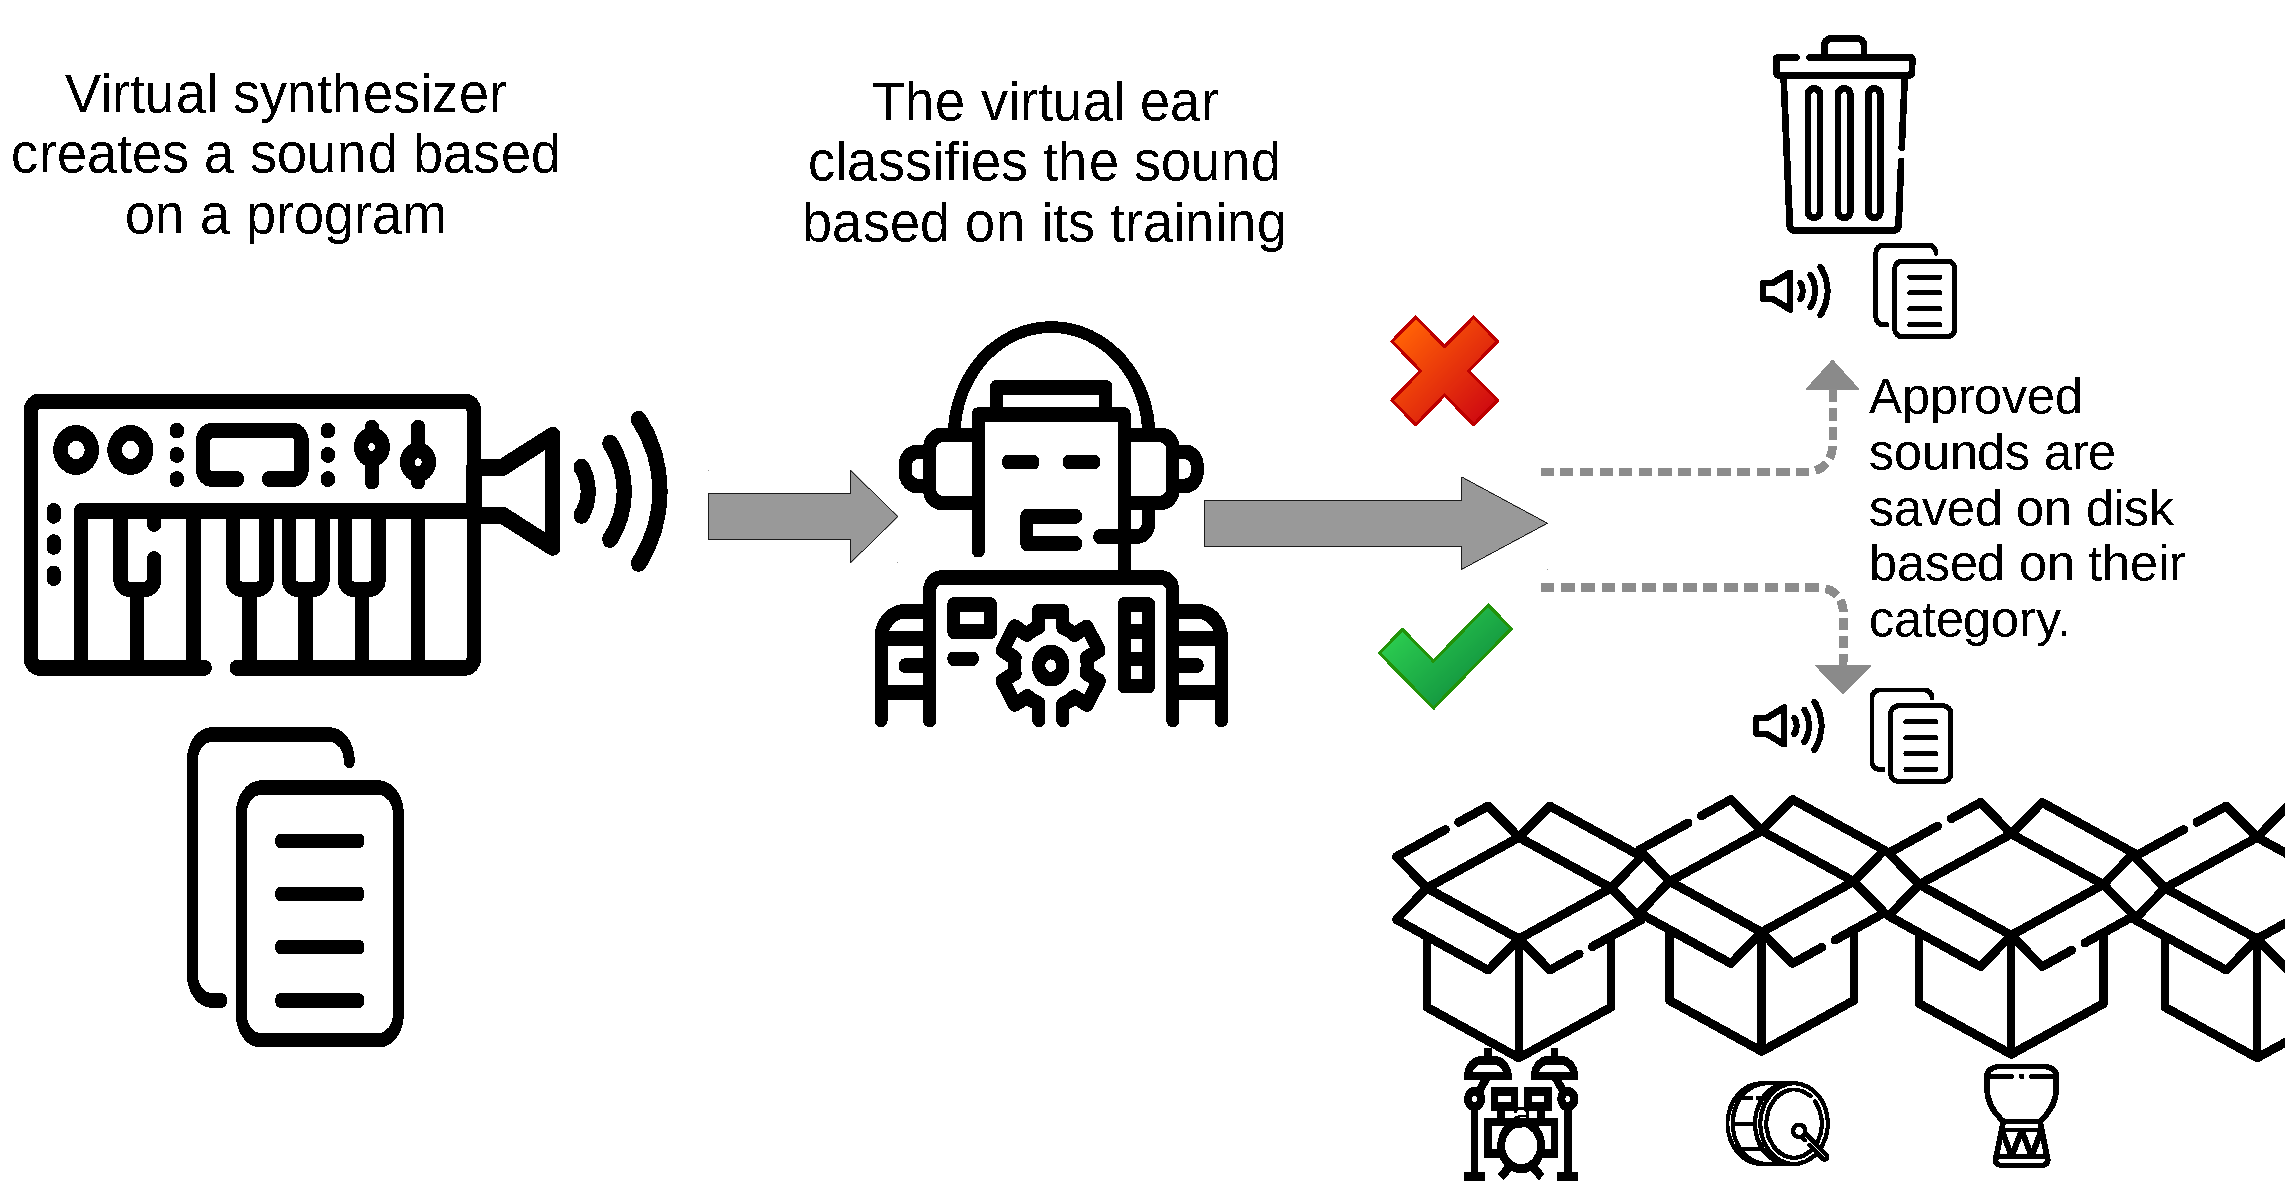
\includegraphics[width=1.1\linewidth]{images/chapter_4/pipeline.pdf}}}
    \end{center}
    \caption{An implementation which allows for easy parallelization when needed. Virtual synthesizer rapidly generates random programs and the corresponding sounds, while the virtual ear will listen to the sounds and determine if they should be categorized as drums and if so, which category of drum do they belong to. 
    }
\label{fig:pipeline_outline}
\end{figure}
\section{Why DSP over ANN Synthesizers?}
 As discussed in Section~\ref{related}, the majority of state of the art works tackling the problem of unsupervised audio generation utilize neural networks for synthesis of audio. Here, rather than using neural networks for sound synthesis, we generate programs for a virtual synthesizer which mainly utilizes additive and subtractive techniques. Our decision is based on the following factors:
\begin{enumerate}[label=(\roman*)]
    \item \textit{Novelty and Creativity}: The goal here is to work with the limitations of any tractable sound source to create its approximations of a given sound category. We seek to create novel sounds via artificial, exploratory creativity. Boden defines this concept as an emergent property of generative work within confined rule sets~\cite{boden2009computer}. An example is the perpetual popularity of 8-bit aesthetics~\cite{collins2007loop}. 
    \item \textit{Interpretability}: Neural networks are often described as black boxes with uninterruptible weights~\cite{basheer2000artificial}. Their highly recursive structure makes modern explanation methods such as saliency maps unreliable~\cite{rudin2019stop}.  
    \item \textit{Speed of Rendering}: Neural network synthesis is costly. Sub 24 kHz sample rates are common in most relevant works~\cite{yamamoto2020parallel,oord2017parallel,aouameur2019neural,ramires2020neural}. This is far below CD quality sampling rates~\cite{reiss2016meta}. At our fixed sampling rate of 48 kHz, synthesizers with 8 submodules can create and save 1 second sounds to hard-disk with an average rendering time of 50 milliseconds\footnote{Using a single process on a Macbook Air 2012 and Ubuntu 18.04}. 
    \item \textit{Flexibility and Scaling}: Probabilistic audio generation is often done sequentially. State of the art, parallel wave generation with GANs requires a fixed amount of rendering time for each time-step~\cite{yamamoto2020parallel}. With our virtual synthesizer, the added footprint of increasing the length of rendered sounds or higher sampling rates is relatively minuscule.  
\end{enumerate}

\section{Virtual Synthesizer Implementation}
\label{virtual_synth_implementation}
 To create sounds, we make use of digital synthesizers capable of rapidly receiving or creating programs, as well as rendering the corresponding sound offline. Classical DSP allows for quick, offline, and parallel generation of audio signals without the usage of GPUs. Pippi\footnote{https://github.com/luvsound/pippi} and SciPy~\cite{jones2001scipy} libraries were extensively used for their DSP functionalities. 

 \begin{figure}[htbp]
    \begin{center}
    % \textbf{Synthesizer SubModule }
    \makebox[\textwidth]{
    \fbox{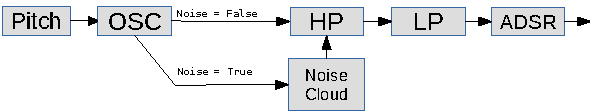
\includegraphics[width=1\linewidth]{images/chapter_3/synthesizer_block.pdf}}}
    \end{center}
    \caption{High level representation of a submodule. Each Synthesizer contains 1 or more submodules. Synthesizer programs set the number of these submodules and their parameters.
    }
\label{fig:submodule}
\end{figure}

 \begin{figure}[htbp]
    \begin{center}
    % \textbf{Synthesizer SubModule }
    \makebox[\textwidth]{
    \fbox{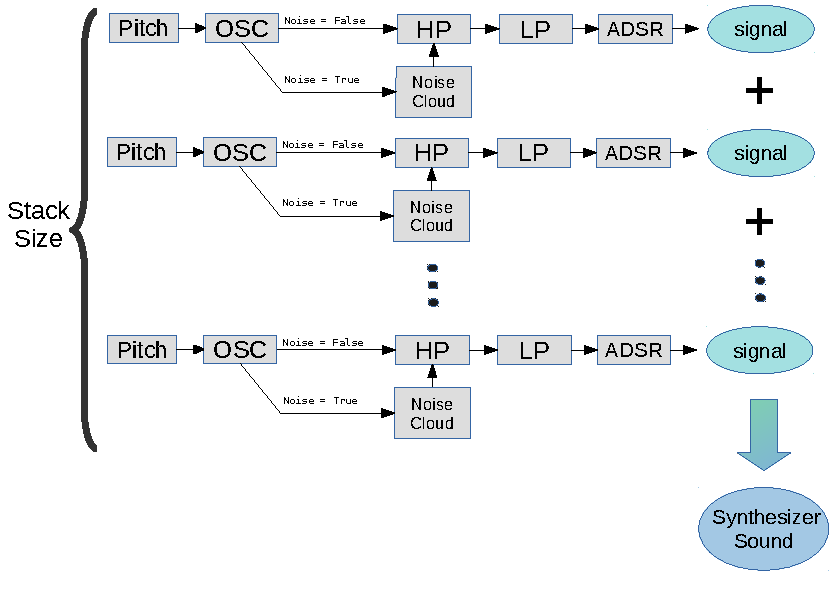
\includegraphics[width=1\linewidth]{images/chapter_3/synthesizer_all_blocks.pdf}}}
    \end{center}
    \caption{The output of the virtual synthesizer is the normalized addition of the output of its submodules. A synthesizer can have any number of submodules. 
    }
\label{fig:synth_modules}
\end{figure}
 The virtual synthesizer contains a set of one or more submodules. Each submodule is a self-contained noise making unit. Submodules have identical structures, but widely different outputs can be achieved depending on the values assigned to their parameters. The output of the virtual synthesizer is the normalized addition of the output of its submodules. As shown in Figure~\ref{fig:synth_modules}, each submodule creates a sound independently, and the results are added and normalized to create the final output. The synthesizer can have any number of submodules. The parameters that dictate the output signal of each submodule as well as the range of values each parameter can take are shown in Table~\ref{table:submodule_params}. We call the number of submodules in each virtual synthesizer the \textit{stack size}. We call the sets of parameter values that characterize a synthesizer's submodules a \textit{program} (analogous to a preset for a VST).  

Since we are interested in short, one-shot percussive sounds, each virtual synthesizer program will generate a 1 second piece of audio. This 1 second limit is over twice the length of the average one-shot drum sample in MixedDB (around 0.4 seconds). Each submodule can make an audio signal with the length of 0.1-1 second, and play it at any point within the 1 second rendering time\footnote{The entire sound must fit within the second, for example, a 0.3 second sound cannot begin playing past 0.7 seconds into the rendering time frame}.
\begin{table}[t!]
\centering
\resizebox{\columnwidth}{!}{\begin{tabular}{ |c|c|c| } 
\hline
Parameters & Value Range & notes and constraints\\
\hline \hline
Attack & 0-3 & A-D-S-R values relative\\
Decay & 0-3 & relative to A-S-R\\
Sustain & 0-3 & relative to A-D-R\\
Release & 0-3 & relative to A-D-S\\
OSC type & sine,square,saw & tone type\\
IsNoise & boolean & whether to \newline use OSC type to generate noise\\
Length & 0-1 second & - \\
StartTime & 0-1 second & Length+Start$<$1\\
Amplitude & 0.1-1 & 1 = max amplitude\\
Pitches(notes) & list of pitches &  range of C0(16.35hz) to B9 \\
HP filter Cutoff & 0-20000hz & -\\
LP filter Cutoff & 20000-HP & never lower than HP cutoff\\
Filter Order & 4,8,16 & butterworth filter order \\
\hline
\end{tabular}}
\caption{Synthesizer submodule parameters. Despite the simplicity of the parameters and efforts at constraining the ranges, the number of parameters that can be randomly chosen for each submodule is in the order of $10^{15}$ }
\label{table:submodule_params}
\end{table}

In Section~\ref{sec:adsr}, we discussed sound envelopes and ADSR parameters, which are used in sound synthesis for modulating the loudness of sounds overtime. Here, each submodule creates its signal at full amplitude before shaping it according to its internal ADSR parameter. Prior to being applied to the signal, each of these parameters is assigned an integer value in the range of 0-3, and normalized relative to the others such that \[ A_{norm} + D_{norm} + S_{norm} + R_{norm} = 1 \] \\ 
Where each value $v_{norm}$ in the $\{A_{norm}, D_{norm},S_{norm},R_{norm}\} $ set is normalized such that:
\begin{align*}
\text{for each $v$ $\epsilon$ \{A,D,S,R\}} \\
v_{norm} = \dfrac{v}{A + D + S + R}
\end{align*}
 The OSC type will determine the wave-shape of the signal. This parameter is limited to three fundamental wave forms: sine waves, square waves and saw waves. We also allow the creation of noise signals, which can imitate timbral characteristics of higher pitched drum samples at a very low computation cost, compared to the addition of thousands of sine waves at various frequencies. If the IsNoise boolean is set to true, the OSC type parameter loses importance as the wave type will be routed through a noise-cloud. 

Each submodule is a monophonic synthesizer. That is, each submodule can play one note (or frequency) at a time. However, quick changes in pitch can occur in drum sound.  To mimic such sounds, synthesizer submodules may slide between 4 different pitches in the 1 second time frame. Each pitch value is a midi note with a frequency and length value. Each submodule accepts a list of 5 consecutive possible pitch values. The submodule will play each note in the list consecutively after normalizing the length values. The pitch notes are played in a portmanteau fashion such that there is no audible gap. This normalization of length values is similar to that of the ADSR values. 

\subsection{How Will The Synthesizer Be Used?}
We use this synthesizer as our source of noise generation. A stack number can be picked randomly, and for each submodule in the stack, the parameter space can be randomly sampled. This gives us a randomly generated~\textit{program}, which is then given to the synthesizer for rendering. These randomly generated sounds can then be listened to in order to find interesting sounds. The goal is to automate the listening procedure for rapid generation of desirable sounds, which are drums in the scope of this project. In the next section, we will discuss the virtual ear, which can automatically listen to the outputs of this synthesizer and separate percussive sounds from non-percussive sounds. 

\end{document}